\section[toc=MC generators]{Monte Carlo generators}

%%%%% BUFFON'S NEEDLE PROBLEM %%%%

\begin{wideslide}{Buffon's needle problem}
\null\vfill

  \twocolumn
  {
    {\it Suppose we have a floor made of parallel strips of wood, each the same width, and we drop a needle onto the floor. What is the probability that the needle will lie across a line between two strips?}
    
    \sep
    
    {\it\hfill Georges-Louis Leclerc,\\\hfill Comte de Buffon\\\hfill 18th century}
  }
  {
    \sep\sep
    \centering\begin{tikzpicture}[node distance = 0cm]
 
  \node (a) [rectH, filled2=pdcolor1, line width = 0] {};
  \node (b) [rectH, notFilled=pdcolor1, line width = 0, right=of a] {};
  \node (c) [rectH, filled2=pdcolor1, line width = 0, right=of b] {};
  \node (d) [rectH, notFilled=pdcolor1, line width = 0, right=of c] {};
  \node (e) [rectH, filled2=pdcolor1, line width = 0, right=of d] {};
  \node (f) [rectH, notFilled=pdcolor1, line width = 0, right=of e] {};
  
  \draw[color = pdcolor7, ultra thick, xshift=0.1cm, yshift=0.0cm, rotate=45] (0,0) -- (0.4,0);
  \draw[color = pdcolor6, ultra thick, xshift=1.4cm, yshift=-0.8cm, rotate=35] (0,0) -- (0.4,0);
  \draw[color = pdcolor7, ultra thick, xshift=2.0cm, yshift=-0.4cm, rotate=-30] (0,0) -- (0.4,0);
  \draw[color = pdcolor6, ultra thick, xshift=2.5cm, yshift=0.6cm, rotate=60] (0,0) -- (0.4,0);
  \draw[color = pdcolor6, ultra thick, xshift=0.8cm, yshift=-0.5cm, rotate=-20] (0,0) -- (0.4,0);
  \draw[color = pdcolor7, ultra thick, xshift=1.1cm, yshift=0.3cm, rotate=15] (0,0) -- (0.4,0);
 
  \node(red) [below=of c, yshift=-0.1cm] {\color{pdcolor7} blue are good};
  \node(blue) [below=of red] {\color{pdcolor6} red are bad};
 
\end{tikzpicture}

  }
  
  \vspace{-10pt}
  \myBoxFullWidth{Monte Carlo without computers}
  
  \twocolumn
  {
    If needle length ($l$) $<$ lines width ($t$):
    
    $$P = \frac{2l}{t\pi}$$
    
    which can be used to estimate $\pi$:
    
    $$\pi = \frac{2l}{tP}$$
  }
  {
    MC experiment was performed by Mario Lazzarini in 1901 by throwing 3408 needles:
    
    $$\pi = \frac{2l \cdot 3408}{t \cdot \#red} = \frac{355}{113} = 3.14159292$$
  }
  
\vfill\null
\end{wideslide}

%%%%% STANISŁAM ULAM %%%%%

\begin{wideslide}[toc = From Solitaire to MC]{From Solitaire to Monte Carlo method}
\null\vfill

    \twocolumn
    {
      \begin{itemize}
	\item Stanis{\l}aw Ulam was a Polish mathematician
	\item He invented the Monte Carlo method while playing solitaire
	\item The method was used in Los Alamos, performed by ENIAC computer
      \end{itemize}  
      
      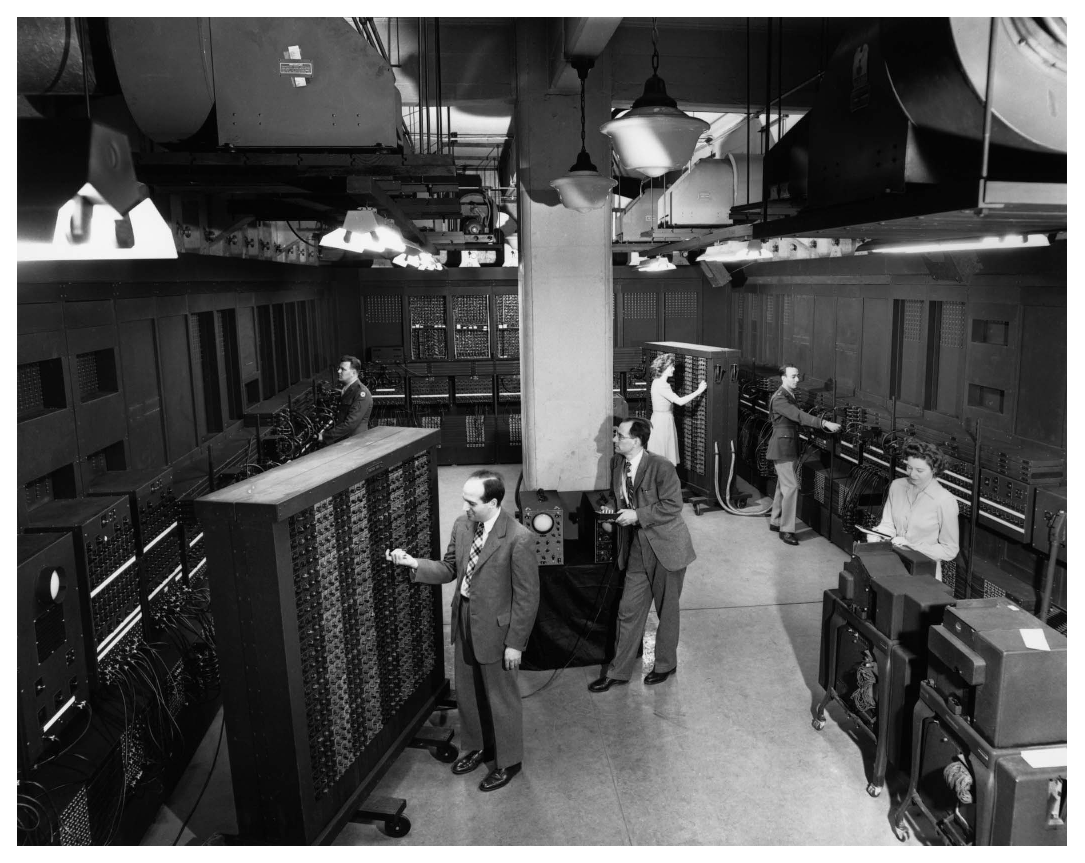
\includegraphics[width=\columnwidth]{img/eniac1946.eps}
    }
    {
      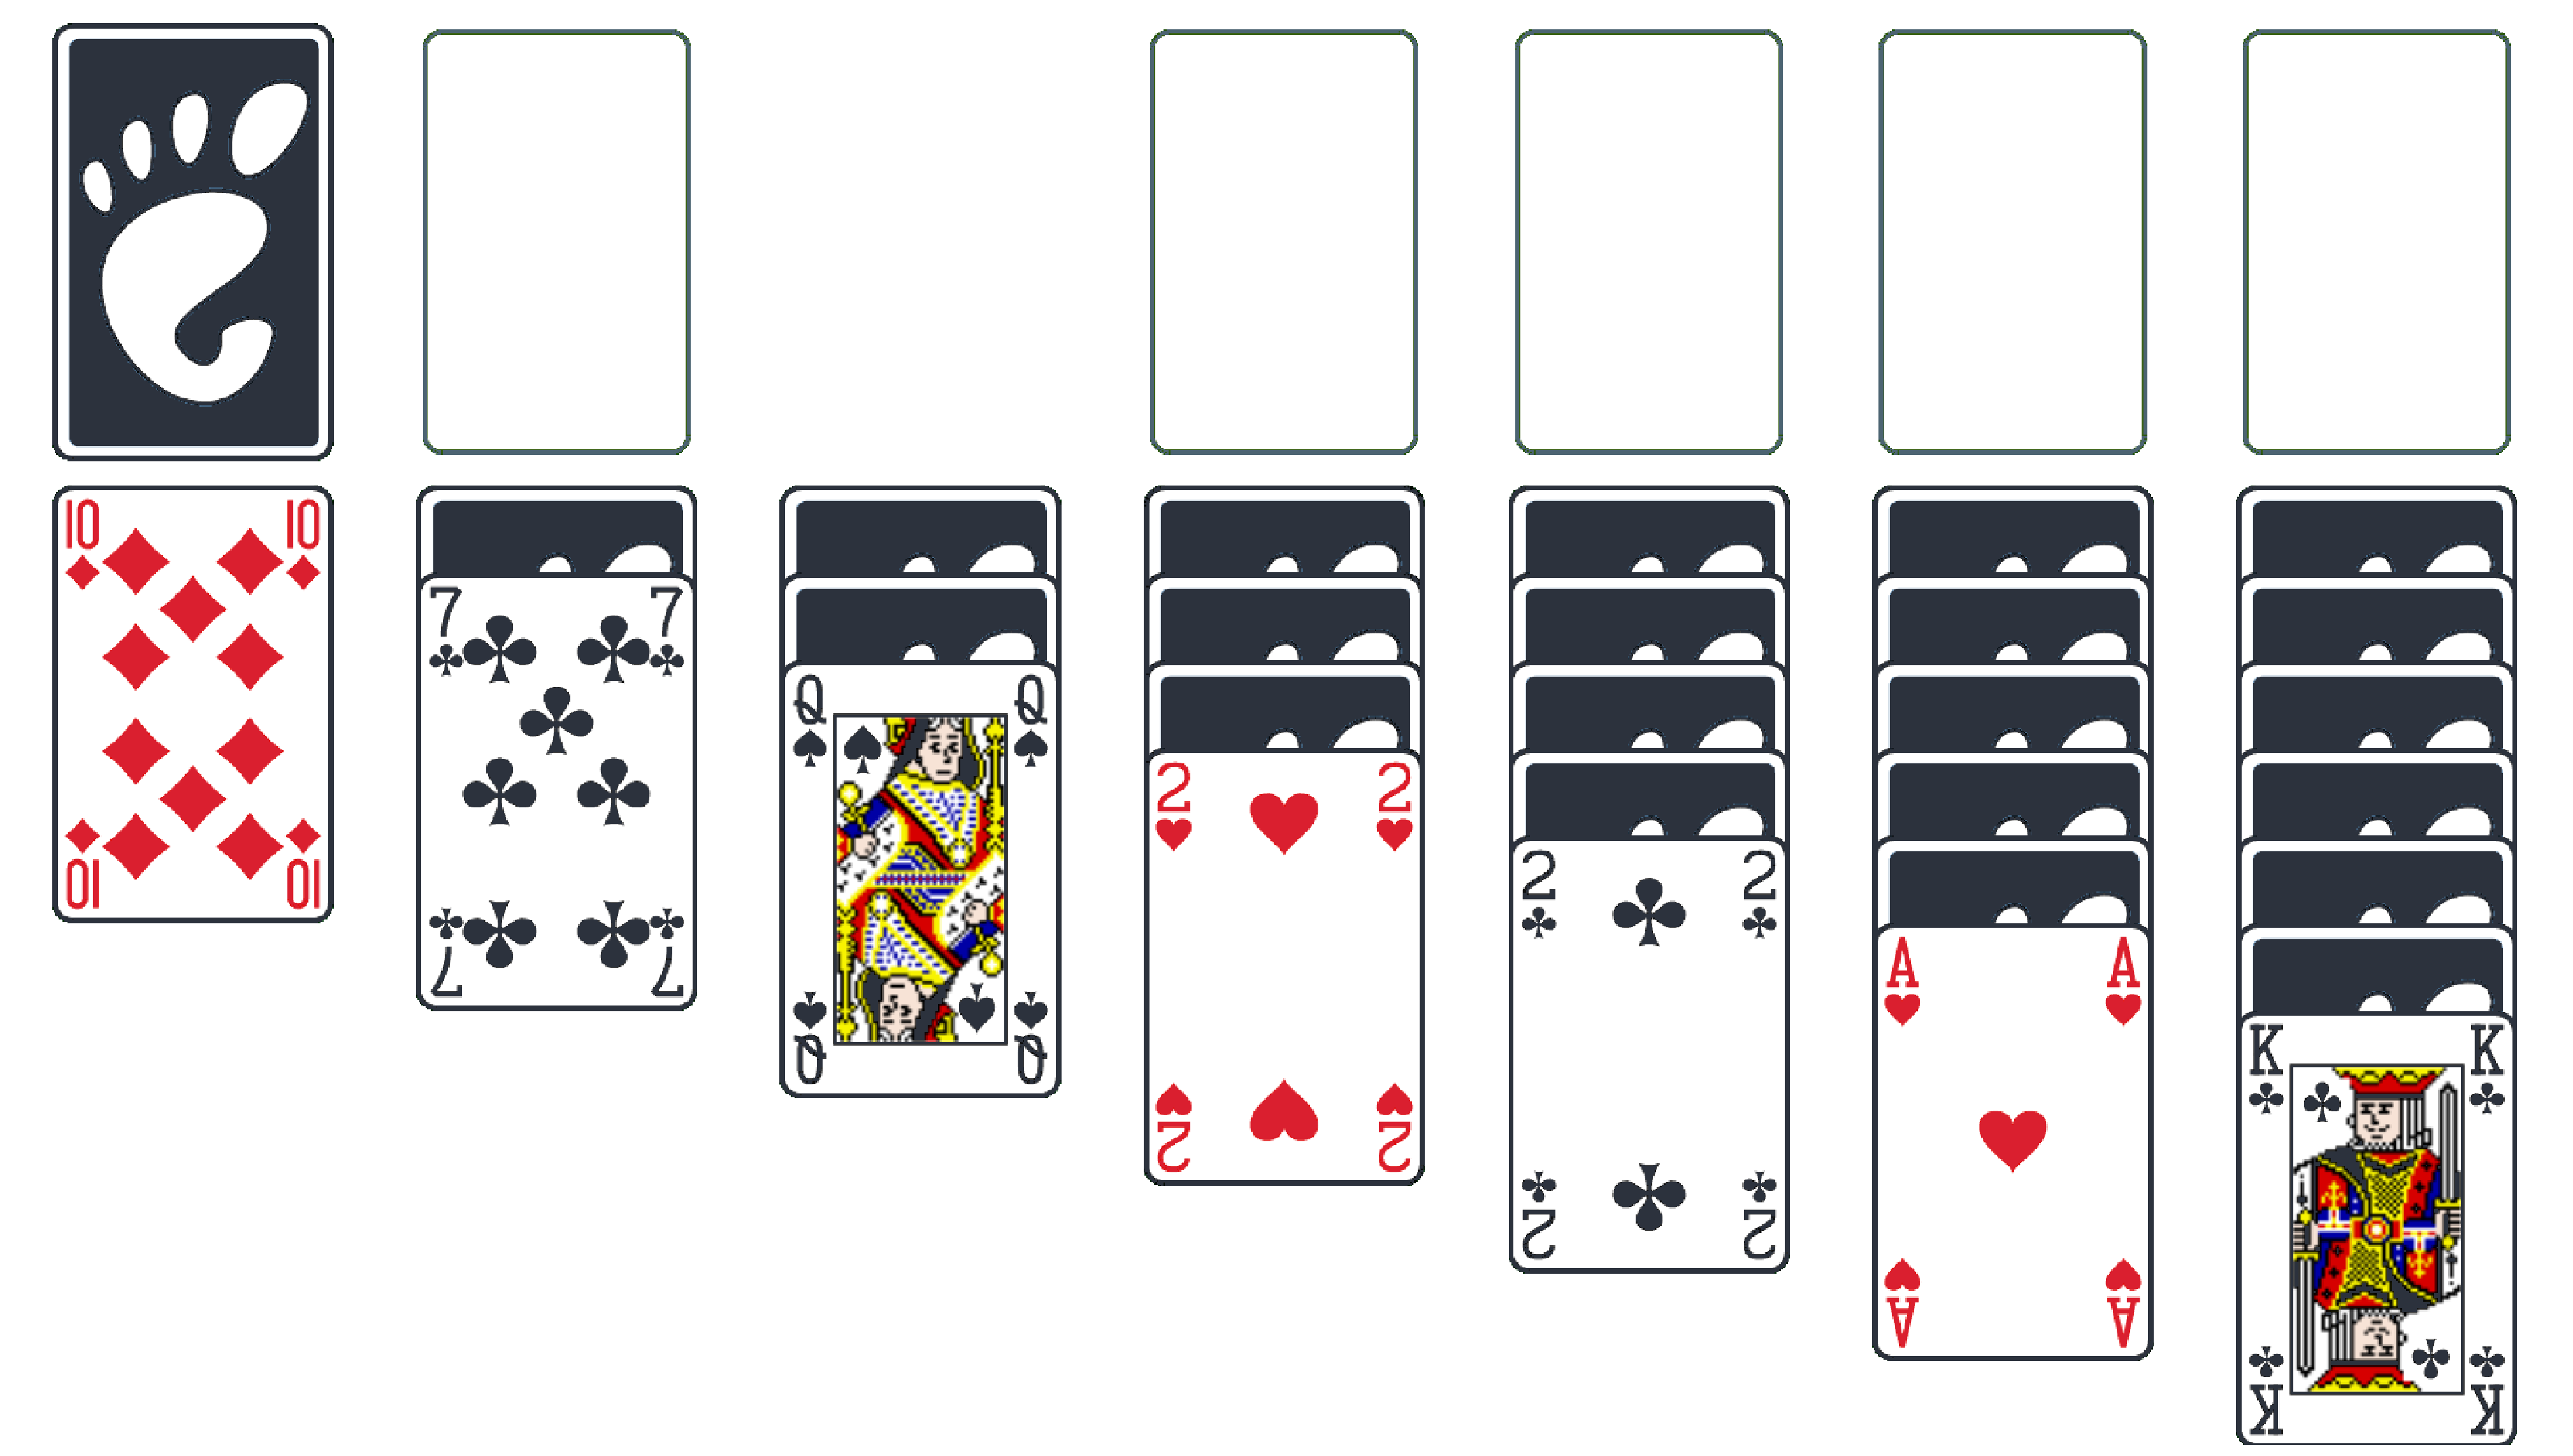
\includegraphics[width=\columnwidth]{img/solitaire.eps}
      \begin{itemize}
	\item What is a probability of success in solitaire?
	\begin{itemize}
	  \item Too complex for an analytical calculations
	  \item Lets try $N = 100$ times and count wins
	  \item With $N \rightarrow \infty$ we are getting closer to correct result
	\end{itemize}
      \end{itemize}
    }
 
\vfill\null
\end{wideslide}

%%%%% MC INTEGRATION: HIT-OR-MISS %%%%%

\begin{slide}[toc=Hit-or-miss method]{MC integration (hit-or-miss method)}
\null\vfill

  Lets do the following integration using MC method:
  
  $$\int_0^1 f(x)dx = \int_0^1 \left(\frac{1}{2}x\right) dx = \left.\frac{1}{2}\frac{x^2}{2}\right|_{0}^{1} = \frac{1}{4}$$

  \twocolumn
  {
    \sep
    \begin{itemize}
     \item take a random point from the $[0,1]\times[0,1]$ square
     \item compare it to your $f(x)$
     \item repeat $N$ times
     \item count $n$ points below the function
     \item you results is given by
     $$\int_0^1 f(x)dx = P_{\square} \cdot \frac{n}{N} = \frac{n}{N}$$
    \end{itemize}
  }
  {
    \usetikzlibrary{calc}

\begin{tikzpicture}

  \draw[>=latex, <->, thick] node[left, yshift = 4cm]{$y$} ++ (0, 4) -- (0, 0) -- node[below, xshift = 2cm]{$x$} ++ (4,0);
  
  \foreach \x in {1,...,200}
  {
    \pgfmathparse{rnd}
    \pgfmathsetmacro{\a}{2.9*\pgfmathresult + 0.05}
    \pgfmathparse{rnd}
    \pgfmathsetmacro{\b}{2.9*\pgfmathresult + 0.05}
    \pgfmathsetmacro{\c}{\a - 2.0 * \b}
        
    \ifthenelse{\lengthtest{\c pt > 0.2 pt}}{\draw[filled, color=pdcolor7] (\a, \b) circle (0.03);}{}
    \ifthenelse{\lengthtest{\c pt < - 0.2 pt}}{\draw[filled, color=pdcolor6] (\a, \b) circle (0.03);}{}
  }

  \draw[ultra thick] (0,0) -- node[yshift = 1.5cm, xshift = 2cm]{$f(x) = \frac{1}{2}x$} ++ (4,2);
  
  \draw[color=pdcolor3, dashed] node[left, yshift = 3cm]{1} ++ (0, 3) -- (3,3) -- node[yshift = -1.75cm]{1} (3, 0);
      
\end{tikzpicture}

  }
  
\vfill\null
\end{slide}

%%%%% MC INTEGRATION: CRUDE METHOD %%%%%

\begin{slide}[toc=Crude method]{MC integration (crude method)}
\null\vfill

  Lets do the following integration using MC method once again:
  
  $$\int_0^1 f(x)dx = \int_0^1 \left(\frac{1}{2}x\right) dx = \left.\frac{1}{2}\frac{x^2}{2}\right|_{0}^{1} = \frac{1}{4}$$
  \twocolumn
  {
    \begin{itemize}
      \item One can approximate integral
      \vspace{-5pt}
      $$\int_a^b f(x) dx \approx \frac{b - a}{N}\sum_{i=1}^{N} f(x_i)$$
     
      where $x_i$ is a random number from $[a, b]$
      
      \item It can be shown that crude method is more accurate than hit-or-miss
      
      \item We will skip the math and look at some comparisons
      
    \end{itemize}
  }
  {
    \usetikzlibrary{calc}

\begin{tikzpicture}

  \draw[>=latex, <->, thick] node[left, yshift = 4cm]{$y$} ++ (0, 4) -- (0, 0) -- node[below, xshift = 2cm]{$x$} ++ (4,0);
  
  \foreach \x in {1,...,14}
  {
    \pgfmathparse{rnd}

    \pgfmathsetmacro{\a}{0.2 * \x + 0.05 + 0.1 * \pgfmathresult - 0.05}
        
    \draw[filled, color=pdcolor7] (\a, 0) circle (0.03);
    
    \draw[thin, color=pdcolor3, dashed] (\a, 0) -- (\a, 0.5*\a);
  }

  \draw[ultra thick] (0,0) -- node[yshift = 1.5cm, xshift = 2cm]{$f(x) = \frac{1}{2}x$} ++ (4,2);
        
\end{tikzpicture}

  }

\vfill\null
\end{slide}

%%%%% HIT-OR-MISS vs CRUDE %%%%%

\begin{emptyslide}{Methods comparison}
\null\vfill

  \twocolumn
  {
    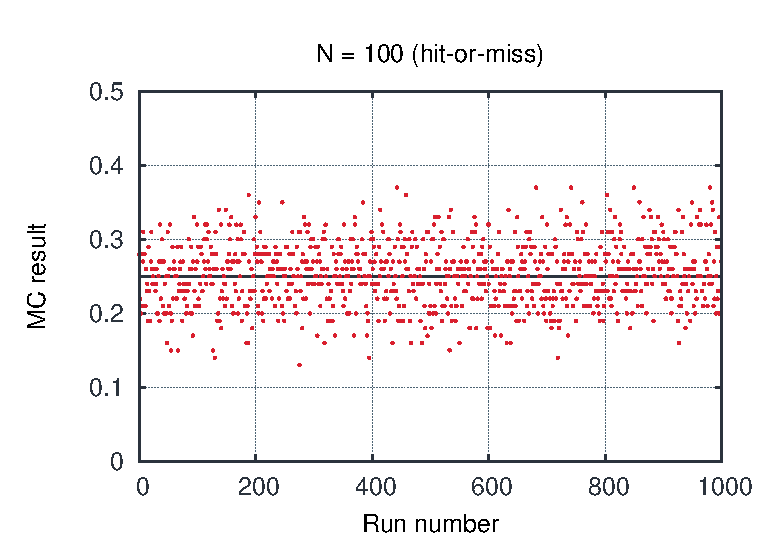
\includegraphics[width=\columnwidth]{img/int100.eps}
    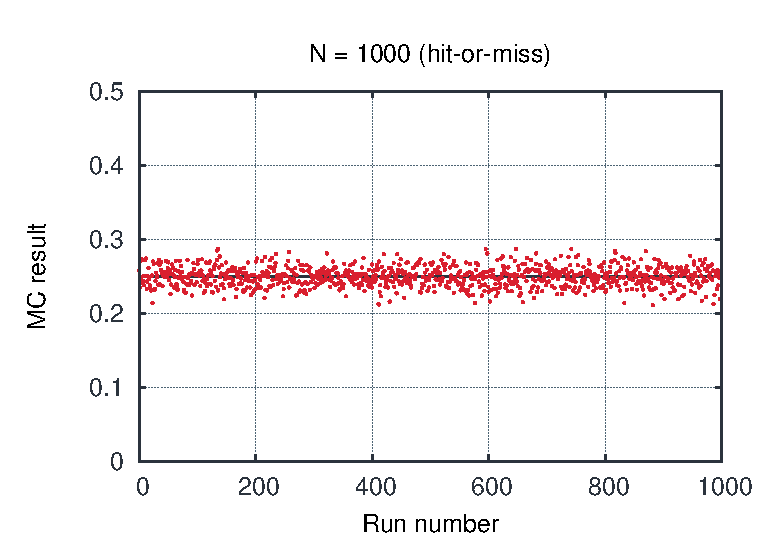
\includegraphics[width=\columnwidth]{img/int1000.eps}
  }
  {
    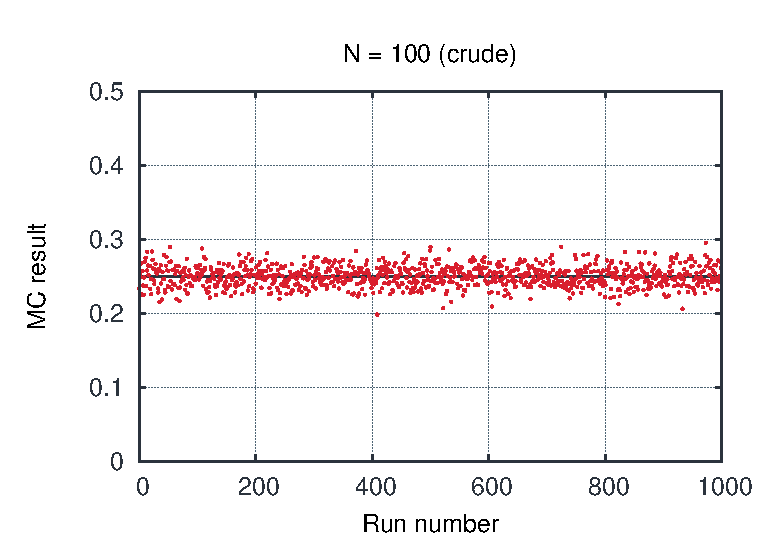
\includegraphics[width=\columnwidth]{img/int2100.eps}
    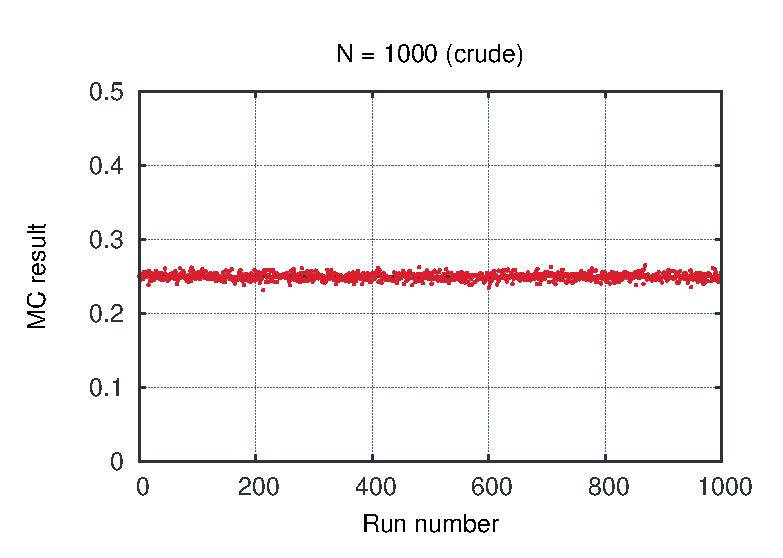
\includegraphics[width=\columnwidth]{img/int21000.eps}
  }

\vfill\null
\end{emptyslide}

%%%%% ACCEPT-REJECT %%%%%

\begin{slide}[toc=Accept-reject]{Acceptance-rejection method}
\null\vfill

  \twocolumn
  {
    \myFrameFullWidth{For generating events \\ according to a distribution.}
    
    \begin{itemize}
      \item Evaluate $f_{max} \geq \mbox{max}(f)$
      \item[] {\it\color{pdcolor3}Note: $f_{max} > \mbox{max}(f)$ will affect performance, but the result will be still correct}
      \item Generate random $x$
      \item Accept $x$ with $P = \frac{f(x)}{f_{max}}$
      \begin{itemize}
	\item generate a random $u$ from $[0, f_{max}]$
	\item accept if $u < f(x)$
      \end{itemize}
    \end{itemize}
  }
  {
    \usetikzlibrary{calc}

\pgfplotsset{every  tick/.style={pdcolor3,}, minor x tick num=1,}

\begin{tikzpicture}

  \begin{axis}[xlabel = {$x$}, ylabel = {$y$}, ylabel near ticks, domain=0:1, scale=0.5, axis lines = left, inner axis line style={>=latex}, ymin = 0, ymax = 0.75, xmin = 0, xmax = 1.1]

    \addplot[mark=none, dashed, color=pdcolor3, thick] coordinates {(0,0.6) (1,0.6) (1,0)};

    \node[above] at (axis cs: 0.5, 0.6) {$f_{max}$};

    \addplot [thick, mark = none, color = pdcolor1] {x*x*x*exp(-x*x)};
    \node[above] at (axis cs: 0.5, 0.3) {\small$f(x) = x^3\cdot e^{-x^2}$};
    
  \end{axis}

\end{tikzpicture}
    \usetikzlibrary{calc}

\pgfplotsset{every  tick/.style={pdcolor3,}, minor x tick num=1,}

\begin{tikzpicture}

  \begin{axis}[xlabel = {$x$}, ylabel = {$y$}, ylabel near ticks, domain=0:1, scale=0.5, axis lines = left, inner axis line style={>=latex}, ymin = 0, ymax = 0.45, xmin = 0, xmax = 1.1]
    
    \addplot [thick, color = pdcolor6] table[x = x, y = y, col sep = space, mark = none] {data/ar.dat};
    \addplot [dashed, mark = none, color = pdcolor1] {x*x*x*exp(-x*x)};
    
  \end{axis}

\end{tikzpicture}
  }

\vfill\null
\end{slide}

%%%%% MC GENERATORS %%%%%

\begin{slide}[toc=MC generators]{Monte Carlo event generators}
\null\vfill

  \rput(1.1\slidewidth, 0.6\slideheight){\scalebox{1.5}{\begin{pspicture}
  \pscircle[linewidth = 0.05, linecolor = pdcolor1](0,0){1}

  \psline[linewidth = 0.05, linecolor = pdcolor4]{->}(-1.6,0)(-1.1,0)
  \psline[linewidth = 0.05, linecolor = pdcolor5]{->}(1.1,0.5)(1.6,0.75)
  \psline[linewidth = 0.05, linecolor = pdcolor5]{->}(1.1,0)(1.6,0)
  \psline[linewidth = 0.05, linecolor = pdcolor5]{->}(1.1,-0.5)(1.6,-0.75)
  
  \rput[c](0,0){\scalebox{0.075}{%LaTeX with PSTricks extensions
%%Creator: inkscape 0.48.4
%%Please note this file requires PSTricks extensions
\psset{xunit=.5pt,yunit=.5pt,runit=.5pt}
\begin{pspicture}(1024,1024)
{
\newrgbcolor{curcolor}{0.12941177 0.14509805 0.19607843}
\pscustom[linestyle=none,fillstyle=solid,fillcolor=curcolor]
{
\newpath
\moveto(476.52942,979.76519)
\curveto(487.77942,998.51519)(514.02942,1021.01519)(532.77942,1021.01519)
\lineto(945.27942,788.51519)
\curveto(952.77942,781.01519)(971.52942,732.26519)(956.52942,713.51519)
\lineto(547.77942,473.51519)
\curveto(536.52942,469.76519)(487.77942,473.51519)(472.77942,511.01519)
\lineto(476.52942,979.76519)
\closepath
}
}
{
\newrgbcolor{curcolor}{0.12941177 0.14509805 0.19607843}
\pscustom[linewidth=3,linecolor=curcolor]
{
\newpath
\moveto(476.52942,979.76519)
\curveto(487.77942,998.51519)(514.02942,1021.01519)(532.77942,1021.01519)
\lineto(945.27942,788.51519)
\curveto(952.77942,781.01519)(971.52942,732.26519)(956.52942,713.51519)
\lineto(547.77942,473.51519)
\curveto(536.52942,469.76519)(487.77942,473.51519)(472.77942,511.01519)
\lineto(476.52942,979.76519)
\closepath
}
}
{
\newrgbcolor{curcolor}{1 1 1}
\pscustom[linestyle=none,fillstyle=solid,fillcolor=curcolor]
{
\newpath
\moveto(517.1383,502.04801)
\curveto(506.42376,483.44891)(488.892,483.44915)(478.17747,502.04825)
\lineto(359.4827,708.08751)
\curveto(348.76859,726.68588)(348.76816,757.11932)(359.4827,775.7184)
\lineto(478.17747,981.75767)
\curveto(488.89172,1000.356275)(506.42418,1000.356275)(517.1383,981.75791)
\lineto(635.83307,775.71865)
\curveto(646.54761,757.11956)(646.54732,726.68588)(635.83307,708.08728)
\lineto(517.1383,502.04801)
\closepath
}
}
{
\newrgbcolor{curcolor}{0.12941177 0.14509805 0.19607843}
\pscustom[linewidth=3.73868561,linecolor=curcolor]
{
\newpath
\moveto(517.1383,502.04801)
\curveto(506.42376,483.44891)(488.892,483.44915)(478.17747,502.04825)
\lineto(359.4827,708.08751)
\curveto(348.76859,726.68588)(348.76816,757.11932)(359.4827,775.7184)
\lineto(478.17747,981.75767)
\curveto(488.89172,1000.356275)(506.42418,1000.356275)(517.1383,981.75791)
\lineto(635.83307,775.71865)
\curveto(646.54761,757.11956)(646.54732,726.68588)(635.83307,708.08728)
\lineto(517.1383,502.04801)
\closepath
}
}
{
\newrgbcolor{curcolor}{0.12941177 0.14509805 0.19607843}
\pscustom[linestyle=none,fillstyle=solid,fillcolor=curcolor]
{
\newpath
\moveto(514.02984324,770.32250396)
\curveto(523.07178558,754.62682324)(523.07178558,729.17909676)(514.02984324,713.48341604)
\curveto(504.98790089,697.78773531)(490.32801581,697.78773531)(481.28607346,713.48341604)
\curveto(472.24413112,729.17909676)(472.24413112,754.62682324)(481.28607346,770.32250396)
\curveto(490.32801581,786.01818469)(504.98790089,786.01818469)(514.02984324,770.32250396)
\closepath
}
}
{
\newrgbcolor{curcolor}{0.12941177 0.14509805 0.19607843}
\pscustom[linewidth=2.67048985,linecolor=curcolor]
{
\newpath
\moveto(514.02984324,770.32250396)
\curveto(523.07178558,754.62682324)(523.07178558,729.17909676)(514.02984324,713.48341604)
\curveto(504.98790089,697.78773531)(490.32801581,697.78773531)(481.28607346,713.48341604)
\curveto(472.24413112,729.17909676)(472.24413112,754.62682324)(481.28607346,770.32250396)
\curveto(490.32801581,786.01818469)(504.98790089,786.01818469)(514.02984324,770.32250396)
\closepath
}
}
{
\newrgbcolor{curcolor}{1 1 1}
\pscustom[linestyle=none,fillstyle=solid,fillcolor=curcolor]
{
\newpath
\moveto(936.13332,746.70165)
\curveto(957.59787,746.72225)(966.36354,731.53907)(955.61352,712.96046)
\lineto(836.52566,507.14816)
\curveto(825.77606,488.57028)(799.42013,473.35319)(777.95558,473.33272)
\lineto(540.17294,473.10577)
\curveto(518.70894,473.08527)(509.9427,488.26883)(520.6923,506.8467)
\lineto(639.78018,712.65902)
\curveto(650.5302,731.23763)(676.88668,746.45421)(698.35068,746.4747)
\lineto(936.13332,746.70165)
\closepath
}
}
{
\newrgbcolor{curcolor}{0.12941177 0.14509805 0.19607843}
\pscustom[linewidth=3.73868561,linecolor=curcolor]
{
\newpath
\moveto(936.13332,746.70165)
\curveto(957.59787,746.72225)(966.36354,731.53907)(955.61352,712.96046)
\lineto(836.52566,507.14816)
\curveto(825.77606,488.57028)(799.42013,473.35319)(777.95558,473.33272)
\lineto(540.17294,473.10577)
\curveto(518.70894,473.08527)(509.9427,488.26883)(520.6923,506.8467)
\lineto(639.78018,712.65902)
\curveto(650.5302,731.23763)(676.88668,746.45421)(698.35068,746.4747)
\lineto(936.13332,746.70165)
\closepath
}
}
{
\newrgbcolor{curcolor}{0.12941177 0.14509805 0.19607843}
\pscustom[linestyle=none,fillstyle=solid,fillcolor=curcolor]
{
\newpath
\moveto(844.51944383,690.21935432)
\curveto(853.59133236,705.89774585)(875.62971231,718.62160859)(893.74354319,718.63889718)
\curveto(911.85737406,718.65618578)(919.1873166,705.96035337)(910.11542807,690.28196184)
\curveto(901.04353955,674.60357031)(879.00515959,661.87970757)(860.89132872,661.86241898)
\curveto(842.77749785,661.84513038)(835.44755531,674.54096278)(844.51944383,690.21935432)
\closepath
}
}
{
\newrgbcolor{curcolor}{0.12941177 0.14509805 0.19607843}
\pscustom[linewidth=2.67048991,linecolor=curcolor]
{
\newpath
\moveto(844.51944383,690.21935432)
\curveto(853.59133236,705.89774585)(875.62971231,718.62160859)(893.74354319,718.63889718)
\curveto(911.85737406,718.65618578)(919.1873166,705.96035337)(910.11542807,690.28196184)
\curveto(901.04353955,674.60357031)(879.00515959,661.87970757)(860.89132872,661.86241898)
\curveto(842.77749785,661.84513038)(835.44755531,674.54096278)(844.51944383,690.21935432)
\closepath
}
}
{
\newrgbcolor{curcolor}{0.12941177 0.14509805 0.19607843}
\pscustom[linestyle=none,fillstyle=solid,fillcolor=curcolor]
{
\newpath
\moveto(659.06885402,690.04235259)
\curveto(668.14074254,705.72074412)(690.1791225,718.44460686)(708.29295337,718.46189545)
\curveto(726.40678424,718.47918404)(733.73672678,705.78335164)(724.66483825,690.10496011)
\curveto(715.59294973,674.42656858)(693.55456977,661.70270584)(675.4407389,661.68541724)
\curveto(657.32690803,661.66812865)(649.99696549,674.36396105)(659.06885402,690.04235259)
\closepath
}
}
{
\newrgbcolor{curcolor}{0.12941177 0.14509805 0.19607843}
\pscustom[linewidth=2.67048991,linecolor=curcolor]
{
\newpath
\moveto(659.06885402,690.04235259)
\curveto(668.14074254,705.72074412)(690.1791225,718.44460686)(708.29295337,718.46189545)
\curveto(726.40678424,718.47918404)(733.73672678,705.78335164)(724.66483825,690.10496011)
\curveto(715.59294973,674.42656858)(693.55456977,661.70270584)(675.4407389,661.68541724)
\curveto(657.32690803,661.66812865)(649.99696549,674.36396105)(659.06885402,690.04235259)
\closepath
}
}
{
\newrgbcolor{curcolor}{0.12941177 0.14509805 0.19607843}
\pscustom[linestyle=none,fillstyle=solid,fillcolor=curcolor]
{
\newpath
\moveto(566.19124479,529.52570903)
\curveto(575.26305576,545.20396653)(597.30124731,557.92772049)(615.41492332,557.94500894)
\curveto(633.52859934,557.96229738)(640.85847921,545.26657352)(631.78666825,529.58831602)
\curveto(622.71485728,513.91005852)(600.67666573,501.18630456)(582.56298971,501.16901611)
\curveto(564.44931369,501.15172767)(557.11943382,513.84745153)(566.19124479,529.52570903)
\closepath
}
}
{
\newrgbcolor{curcolor}{0.12941177 0.14509805 0.19607843}
\pscustom[linewidth=2.67048991,linecolor=curcolor]
{
\newpath
\moveto(566.19124479,529.52570903)
\curveto(575.26305576,545.20396653)(597.30124731,557.92772049)(615.41492332,557.94500894)
\curveto(633.52859934,557.96229738)(640.85847921,545.26657352)(631.78666825,529.58831602)
\curveto(622.71485728,513.91005852)(600.67666573,501.18630456)(582.56298971,501.16901611)
\curveto(564.44931369,501.15172767)(557.11943382,513.84745153)(566.19124479,529.52570903)
\closepath
}
}
{
\newrgbcolor{curcolor}{0.12941177 0.14509805 0.19607843}
\pscustom[linestyle=none,fillstyle=solid,fillcolor=curcolor]
{
\newpath
\moveto(705.35499371,609.87241006)
\curveto(714.42688223,625.55080159)(736.46526219,638.27466434)(754.57909306,638.29195293)
\curveto(772.69292393,638.30924152)(780.02286647,625.61340912)(770.95097794,609.93501759)
\curveto(761.87908942,594.25662605)(739.84070946,581.53276331)(721.72687859,581.51547472)
\curveto(703.61304772,581.49818613)(696.28310518,594.19401853)(705.35499371,609.87241006)
\closepath
}
}
{
\newrgbcolor{curcolor}{0.12941177 0.14509805 0.19607843}
\pscustom[linewidth=2.67048991,linecolor=curcolor]
{
\newpath
\moveto(705.35499371,609.87241006)
\curveto(714.42688223,625.55080159)(736.46526219,638.27466434)(754.57909306,638.29195293)
\curveto(772.69292393,638.30924152)(780.02286647,625.61340912)(770.95097794,609.93501759)
\curveto(761.87908942,594.25662605)(739.84070946,581.53276331)(721.72687859,581.51547472)
\curveto(703.61304772,581.49818613)(696.28310518,594.19401853)(705.35499371,609.87241006)
\closepath
}
}
{
\newrgbcolor{curcolor}{0.12941177 0.14509805 0.19607843}
\pscustom[linestyle=none,fillstyle=solid,fillcolor=curcolor]
{
\newpath
\moveto(751.64078083,529.70258469)
\curveto(760.71270813,545.38104323)(782.75118229,558.10496037)(800.86509059,558.12224903)
\curveto(818.97899889,558.1395377)(826.30897276,545.44365103)(817.23704546,529.76519248)
\curveto(808.16511816,514.08673393)(786.126644,501.3628168)(768.0127357,501.34552813)
\curveto(749.89882739,501.32823947)(742.56885352,514.02412614)(751.64078083,529.70258469)
\closepath
}
}
{
\newrgbcolor{curcolor}{0.12941177 0.14509805 0.19607843}
\pscustom[linewidth=2.67048991,linecolor=curcolor]
{
\newpath
\moveto(751.64078083,529.70258469)
\curveto(760.71270813,545.38104323)(782.75118229,558.10496037)(800.86509059,558.12224903)
\curveto(818.97899889,558.1395377)(826.30897276,545.44365103)(817.23704546,529.76519248)
\curveto(808.16511816,514.08673393)(786.126644,501.3628168)(768.0127357,501.34552813)
\curveto(749.89882739,501.32823947)(742.56885352,514.02412614)(751.64078083,529.70258469)
\closepath
}
}
{
\newrgbcolor{curcolor}{1 1 1}
\pscustom[linestyle=none,fillstyle=solid,fillcolor=curcolor]
{
\newpath
\moveto(514.94154,986.827505)
\curveto(504.19152,1005.4061)(512.95761,1020.588935)(534.42218,1020.568445)
\lineto(772.20482,1020.341495)
\curveto(793.66853,1020.321095)(820.02488,1005.10466)(830.7749,986.52605)
\lineto(949.86276,780.71375)
\curveto(960.61251,762.13564)(951.84627,746.95207)(930.38256,746.97256)
\lineto(692.59992,747.19951)
\curveto(671.13535,747.22)(644.77916,762.43708)(634.02942,781.01519)
\lineto(514.94154,986.827505)
\closepath
}
}
{
\newrgbcolor{curcolor}{0.12941177 0.14509805 0.19607843}
\pscustom[linewidth=3.73868561,linecolor=curcolor]
{
\newpath
\moveto(514.94154,986.827505)
\curveto(504.19152,1005.4061)(512.95761,1020.588935)(534.42218,1020.568445)
\lineto(772.20482,1020.341495)
\curveto(793.66853,1020.321095)(820.02488,1005.10466)(830.7749,986.52605)
\lineto(949.86276,780.71375)
\curveto(960.61251,762.13564)(951.84627,746.95207)(930.38256,746.97256)
\lineto(692.59992,747.19951)
\curveto(671.13535,747.22)(644.77916,762.43708)(634.02942,781.01519)
\lineto(514.94154,986.827505)
\closepath
}
}
{
\newrgbcolor{curcolor}{0.12941177 0.14509805 0.19607843}
\pscustom[linestyle=none,fillstyle=solid,fillcolor=curcolor]
{
\newpath
\moveto(609.663603,935.72872148)
\curveto(591.54977213,935.74601007)(569.51139217,948.46987282)(560.43950365,964.14826435)
\curveto(551.36761513,979.82665588)(558.69755766,992.52248828)(576.81138854,992.50519969)
\curveto(594.92521941,992.4879111)(616.96359937,979.76404835)(626.03548789,964.08565682)
\curveto(635.10737641,948.40726529)(627.77743388,935.71143289)(609.663603,935.72872148)
\closepath
}
}
{
\newrgbcolor{curcolor}{0.12941177 0.14509805 0.19607843}
\pscustom[linewidth=2.67048991,linecolor=curcolor]
{
\newpath
\moveto(609.663603,935.72872148)
\curveto(591.54977213,935.74601007)(569.51139217,948.46987282)(560.43950365,964.14826435)
\curveto(551.36761513,979.82665588)(558.69755766,992.52248828)(576.81138854,992.50519969)
\curveto(594.92521941,992.4879111)(616.96359937,979.76404835)(626.03548789,964.08565682)
\curveto(635.10737641,948.40726529)(627.77743388,935.71143289)(609.663603,935.72872148)
\closepath
}
}
{
\newrgbcolor{curcolor}{0.12941177 0.14509805 0.19607843}
\pscustom[linestyle=none,fillstyle=solid,fillcolor=curcolor]
{
\newpath
\moveto(702.54219337,775.21231955)
\curveto(684.4283625,775.22960814)(662.38998254,787.95347088)(653.31809402,803.63186241)
\curveto(644.24620549,819.31025395)(651.57614803,832.00608635)(669.6899789,831.98879776)
\curveto(687.80380977,831.97150916)(709.84218973,819.24764642)(718.91407825,803.56925489)
\curveto(727.98596678,787.89086336)(720.65602424,775.19503096)(702.54219337,775.21231955)
\closepath
}
}
{
\newrgbcolor{curcolor}{0.12941177 0.14509805 0.19607843}
\pscustom[linewidth=2.67048991,linecolor=curcolor]
{
\newpath
\moveto(702.54219337,775.21231955)
\curveto(684.4283625,775.22960814)(662.38998254,787.95347088)(653.31809402,803.63186241)
\curveto(644.24620549,819.31025395)(651.57614803,832.00608635)(669.6899789,831.98879776)
\curveto(687.80380977,831.97150916)(709.84218973,819.24764642)(718.91407825,803.56925489)
\curveto(727.98596678,787.89086336)(720.65602424,775.19503096)(702.54219337,775.21231955)
\closepath
}
}
{
\newrgbcolor{curcolor}{0.12941177 0.14509805 0.19607843}
\pscustom[linestyle=none,fillstyle=solid,fillcolor=curcolor]
{
\newpath
\moveto(887.99250187,775.03628832)
\curveto(869.87882585,775.05357676)(847.8406343,787.77733073)(838.76882333,803.45558823)
\curveto(829.69701236,819.13384572)(837.02689224,831.82956959)(855.14056825,831.81228114)
\curveto(873.25424427,831.7949927)(895.29243582,819.07123873)(904.36424679,803.39298123)
\curveto(913.43605776,787.71472374)(906.10617788,775.01899988)(887.99250187,775.03628832)
\closepath
}
}
{
\newrgbcolor{curcolor}{0.12941177 0.14509805 0.19607843}
\pscustom[linewidth=2.67048991,linecolor=curcolor]
{
\newpath
\moveto(887.99250187,775.03628832)
\curveto(869.87882585,775.05357676)(847.8406343,787.77733073)(838.76882333,803.45558823)
\curveto(829.69701236,819.13384572)(837.02689224,831.82956959)(855.14056825,831.81228114)
\curveto(873.25424427,831.7949927)(895.29243582,819.07123873)(904.36424679,803.39298123)
\curveto(913.43605776,787.71472374)(906.10617788,775.01899988)(887.99250187,775.03628832)
\closepath
}
}
{
\newrgbcolor{curcolor}{0.12941177 0.14509805 0.19607843}
\pscustom[linestyle=none,fillstyle=solid,fillcolor=curcolor]
{
\newpath
\moveto(795.11454758,935.55184069)
\curveto(777.00063927,935.56912936)(754.96216511,948.29304649)(745.89023781,963.97150504)
\curveto(736.81831051,979.64996359)(744.14828438,992.34585026)(762.26219268,992.32856159)
\curveto(780.37610098,992.31127293)(802.41457514,979.58735579)(811.48650244,963.90889724)
\curveto(820.55842975,948.23043869)(813.22845588,935.53455203)(795.11454758,935.55184069)
\closepath
}
}
{
\newrgbcolor{curcolor}{0.12941177 0.14509805 0.19607843}
\pscustom[linewidth=2.67048991,linecolor=curcolor]
{
\newpath
\moveto(795.11454758,935.55184069)
\curveto(777.00063927,935.56912936)(754.96216511,948.29304649)(745.89023781,963.97150504)
\curveto(736.81831051,979.64996359)(744.14828438,992.34585026)(762.26219268,992.32856159)
\curveto(780.37610098,992.31127293)(802.41457514,979.58735579)(811.48650244,963.90889724)
\curveto(820.55842975,948.23043869)(813.22845588,935.53455203)(795.11454758,935.55184069)
\closepath
}
}
{
\newrgbcolor{curcolor}{0.12941177 0.14509805 0.19607843}
\pscustom[linestyle=none,fillstyle=solid,fillcolor=curcolor]
{
\newpath
\moveto(654.69727,487.8886)
\curveto(673.44727,476.6386)(695.94727,450.3886)(695.94727,431.6386)
\lineto(454.70688,13.6148)
\curveto(444.71994,7.4401)(423.08878,-4.9951)(392.3516,5.6702)
\lineto(148.44727,416.6386)
\curveto(144.69727,427.8886)(148.44727,476.6386)(185.94727,491.6386)
\lineto(654.69727,487.8886)
\closepath
}
}
{
\newrgbcolor{curcolor}{0.12941177 0.14509805 0.19607843}
\pscustom[linewidth=3,linecolor=curcolor]
{
\newpath
\moveto(654.69727,487.8886)
\curveto(673.44727,476.6386)(695.94727,450.3886)(695.94727,431.6386)
\lineto(454.70688,13.6148)
\curveto(444.71994,7.4401)(423.08878,-4.9951)(392.3516,5.6702)
\lineto(148.44727,416.6386)
\curveto(144.69727,427.8886)(148.44727,476.6386)(185.94727,491.6386)
\lineto(654.69727,487.8886)
\closepath
}
}
{
\newrgbcolor{curcolor}{1 1 1}
\pscustom[linestyle=none,fillstyle=solid,fillcolor=curcolor]
{
\newpath
\moveto(176.98009,447.27972)
\curveto(158.38099,457.99426)(158.38123,475.52602)(176.98033,486.24056)
\lineto(383.01959,604.93533)
\curveto(401.61796,615.64944)(432.0514,615.64986)(450.65049,604.93533)
\lineto(656.68975,486.24056)
\curveto(675.28836,475.52631)(675.28836,457.99384)(656.68999,447.27972)
\lineto(450.65073,328.58496)
\curveto(432.05164,317.87042)(401.61796,317.8707)(383.01935,328.58496)
\lineto(176.98009,447.27972)
\closepath
}
}
{
\newrgbcolor{curcolor}{0.12941177 0.14509805 0.19607843}
\pscustom[linewidth=3.73868585,linecolor=curcolor]
{
\newpath
\moveto(176.98009,447.27972)
\curveto(158.38099,457.99426)(158.38123,475.52602)(176.98033,486.24056)
\lineto(383.01959,604.93533)
\curveto(401.61796,615.64944)(432.0514,615.64986)(450.65049,604.93533)
\lineto(656.68975,486.24056)
\curveto(675.28836,475.52631)(675.28836,457.99384)(656.68999,447.27972)
\lineto(450.65073,328.58496)
\curveto(432.05164,317.87042)(401.61796,317.8707)(383.01935,328.58496)
\lineto(176.98009,447.27972)
\closepath
}
}
{
\newrgbcolor{curcolor}{0.12941177 0.14509805 0.19607843}
\pscustom[linestyle=none,fillstyle=solid,fillcolor=curcolor]
{
\newpath
\moveto(445.25458396,450.38818676)
\curveto(429.55890324,441.34624442)(404.11117676,441.34624442)(388.41549604,450.38818676)
\curveto(372.71981531,459.43012911)(372.71981531,474.09001419)(388.41549604,483.13195654)
\curveto(404.11117676,492.17389888)(429.55890324,492.17389888)(445.25458396,483.13195654)
\curveto(460.95026469,474.09001419)(460.95026469,459.43012911)(445.25458396,450.38818676)
\closepath
}
}
{
\newrgbcolor{curcolor}{0.12941177 0.14509805 0.19607843}
\pscustom[linewidth=2.67048985,linecolor=curcolor]
{
\newpath
\moveto(445.25458396,450.38818676)
\curveto(429.55890324,441.34624442)(404.11117676,441.34624442)(388.41549604,450.38818676)
\curveto(372.71981531,459.43012911)(372.71981531,474.09001419)(388.41549604,483.13195654)
\curveto(404.11117676,492.17389888)(429.55890324,492.17389888)(445.25458396,483.13195654)
\curveto(460.95026469,474.09001419)(460.95026469,459.43012911)(445.25458396,450.38818676)
\closepath
}
}
{
\newrgbcolor{curcolor}{1 1 1}
\pscustom[linestyle=none,fillstyle=solid,fillcolor=curcolor]
{
\newpath
\moveto(421.63374,27.74233)
\curveto(421.65424,6.2778)(406.47115,-2.4879)(387.89255,8.2621)
\lineto(182.08024,127.35)
\curveto(163.50237,138.0996)(148.28528,164.45552)(148.2648,185.92008)
\lineto(148.03785,423.70272)
\curveto(148.01735,445.16671)(163.20092,453.93294)(181.7788,443.18334)
\lineto(387.5911,324.09547)
\curveto(406.16971,313.34545)(421.38631,286.98897)(421.40679,265.52497)
\lineto(421.63374,27.74233)
\closepath
}
}
{
\newrgbcolor{curcolor}{0.12941177 0.14509805 0.19607843}
\pscustom[linewidth=3.73868585,linecolor=curcolor]
{
\newpath
\moveto(421.63374,27.74233)
\curveto(421.65424,6.2778)(406.47115,-2.4879)(387.89255,8.2621)
\lineto(182.08024,127.35)
\curveto(163.50237,138.0996)(148.28528,164.45552)(148.2648,185.92008)
\lineto(148.03785,423.70272)
\curveto(148.01735,445.16671)(163.20092,453.93294)(181.7788,443.18334)
\lineto(387.5911,324.09547)
\curveto(406.16971,313.34545)(421.38631,286.98897)(421.40679,265.52497)
\lineto(421.63374,27.74233)
\closepath
}
}
{
\newrgbcolor{curcolor}{0.12941177 0.14509805 0.19607843}
\pscustom[linestyle=none,fillstyle=solid,fillcolor=curcolor]
{
\newpath
\moveto(365.15143432,119.35620617)
\curveto(380.82982585,110.28431764)(393.55368859,88.24593769)(393.57097718,70.13210681)
\curveto(393.58826578,52.01827594)(380.89243337,44.6883334)(365.21404184,53.76022193)
\curveto(349.53565031,62.83211045)(336.81178757,84.87049041)(336.79449898,102.98432128)
\curveto(336.77721038,121.09815215)(349.47304278,128.42809469)(365.15143432,119.35620617)
\closepath
}
}
{
\newrgbcolor{curcolor}{0.12941177 0.14509805 0.19607843}
\pscustom[linewidth=2.67048991,linecolor=curcolor]
{
\newpath
\moveto(365.15143432,119.35620617)
\curveto(380.82982585,110.28431764)(393.55368859,88.24593769)(393.57097718,70.13210681)
\curveto(393.58826578,52.01827594)(380.89243337,44.6883334)(365.21404184,53.76022193)
\curveto(349.53565031,62.83211045)(336.81178757,84.87049041)(336.79449898,102.98432128)
\curveto(336.77721038,121.09815215)(349.47304278,128.42809469)(365.15143432,119.35620617)
\closepath
}
}
{
\newrgbcolor{curcolor}{0.12941177 0.14509805 0.19607843}
\pscustom[linestyle=none,fillstyle=solid,fillcolor=curcolor]
{
\newpath
\moveto(204.45778903,397.68440521)
\curveto(220.13604653,388.61259424)(232.85980049,366.57440269)(232.87708894,348.46072668)
\curveto(232.89437738,330.34705066)(220.19865352,323.01717079)(204.52039602,332.08898175)
\curveto(188.84213852,341.16079272)(176.11838456,363.19898427)(176.10109611,381.31266029)
\curveto(176.08380767,399.42633631)(188.77953153,406.75621618)(204.45778903,397.68440521)
\closepath
}
}
{
\newrgbcolor{curcolor}{0.12941177 0.14509805 0.19607843}
\pscustom[linewidth=2.67048991,linecolor=curcolor]
{
\newpath
\moveto(204.45778903,397.68440521)
\curveto(220.13604653,388.61259424)(232.85980049,366.57440269)(232.87708894,348.46072668)
\curveto(232.89437738,330.34705066)(220.19865352,323.01717079)(204.52039602,332.08898175)
\curveto(188.84213852,341.16079272)(176.11838456,363.19898427)(176.10109611,381.31266029)
\curveto(176.08380767,399.42633631)(188.77953153,406.75621618)(204.45778903,397.68440521)
\closepath
}
}
{
\newrgbcolor{curcolor}{1 1 1}
\pscustom[linestyle=none,fillstyle=solid,fillcolor=curcolor]
{
\newpath
\moveto(661.75958,449.47647)
\curveto(680.33819,460.2265)(695.52102,451.4604)(695.50053,429.99585)
\lineto(695.27358,192.21321)
\curveto(695.25308,170.74949)(680.03674,144.39315)(661.45814,133.64313)
\lineto(455.64583,14.5553)
\curveto(437.06771,3.8055)(421.88415,12.5717)(421.90464,34.03546)
\lineto(422.13159,271.8181)
\curveto(422.15209,293.28266)(437.36916,319.63886)(455.94728,330.3886)
\lineto(661.75958,449.47647)
\closepath
}
}
{
\newrgbcolor{curcolor}{0.12941177 0.14509805 0.19607843}
\pscustom[linewidth=3.73868585,linecolor=curcolor]
{
\newpath
\moveto(661.75958,449.47647)
\curveto(680.33819,460.2265)(695.52102,451.4604)(695.50053,429.99585)
\lineto(695.27358,192.21321)
\curveto(695.25308,170.74949)(680.03674,144.39315)(661.45814,133.64313)
\lineto(455.64583,14.5553)
\curveto(437.06771,3.8055)(421.88415,12.5717)(421.90464,34.03546)
\lineto(422.13159,271.8181)
\curveto(422.15209,293.28266)(437.36916,319.63886)(455.94728,330.3886)
\lineto(661.75958,449.47647)
\closepath
}
}
{
\newrgbcolor{curcolor}{0.12941177 0.14509805 0.19607843}
\pscustom[linestyle=none,fillstyle=solid,fillcolor=curcolor]
{
\newpath
\moveto(610.66080648,354.754417)
\curveto(610.67809507,372.86824787)(623.40195782,394.90662783)(639.08034935,403.97851635)
\curveto(654.75874088,413.05040487)(667.45457328,405.72046234)(667.43728469,387.60663146)
\curveto(667.4199961,369.49280059)(654.69613335,347.45442063)(639.01774182,338.38253211)
\curveto(623.33935029,329.31064359)(610.64351789,336.64058612)(610.66080648,354.754417)
\closepath
}
}
{
\newrgbcolor{curcolor}{0.12941177 0.14509805 0.19607843}
\pscustom[linewidth=2.67048991,linecolor=curcolor]
{
\newpath
\moveto(610.66080648,354.754417)
\curveto(610.67809507,372.86824787)(623.40195782,394.90662783)(639.08034935,403.97851635)
\curveto(654.75874088,413.05040487)(667.45457328,405.72046234)(667.43728469,387.60663146)
\curveto(667.4199961,369.49280059)(654.69613335,347.45442063)(639.01774182,338.38253211)
\curveto(623.33935029,329.31064359)(610.64351789,336.64058612)(610.66080648,354.754417)
\closepath
}
}
{
\newrgbcolor{curcolor}{0.12941177 0.14509805 0.19607843}
\pscustom[linestyle=none,fillstyle=solid,fillcolor=curcolor]
{
\newpath
\moveto(449.96837332,76.42551813)
\curveto(449.98566176,94.53919415)(462.70941573,116.5773857)(478.38767323,125.64919667)
\curveto(494.06593072,134.72100764)(506.76165459,127.39112776)(506.74436614,109.27745175)
\curveto(506.7270777,91.16377573)(494.00332373,69.12558418)(478.32506623,60.05377321)
\curveto(462.64680874,50.98196224)(449.95108488,58.31184212)(449.96837332,76.42551813)
\closepath
}
}
{
\newrgbcolor{curcolor}{0.12941177 0.14509805 0.19607843}
\pscustom[linewidth=2.67048991,linecolor=curcolor]
{
\newpath
\moveto(449.96837332,76.42551813)
\curveto(449.98566176,94.53919415)(462.70941573,116.5773857)(478.38767323,125.64919667)
\curveto(494.06593072,134.72100764)(506.76165459,127.39112776)(506.74436614,109.27745175)
\curveto(506.7270777,91.16377573)(494.00332373,69.12558418)(478.32506623,60.05377321)
\curveto(462.64680874,50.98196224)(449.95108488,58.31184212)(449.96837332,76.42551813)
\closepath
}
}
{
\newrgbcolor{curcolor}{0.12941177 0.14509805 0.19607843}
\pscustom[linestyle=none,fillstyle=solid,fillcolor=curcolor]
{
\newpath
\moveto(530.31434707,215.58968694)
\curveto(530.33163566,233.70351781)(543.05549841,255.74189777)(558.73388994,264.81378629)
\curveto(574.41228147,273.88567482)(587.10811387,266.55573228)(587.09082528,248.44190141)
\curveto(587.07353669,230.32807054)(574.34967395,208.28969058)(558.67128241,199.21780206)
\curveto(542.99289088,190.14591353)(530.29705848,197.47585607)(530.31434707,215.58968694)
\closepath
}
}
{
\newrgbcolor{curcolor}{0.12941177 0.14509805 0.19607843}
\pscustom[linewidth=2.67048991,linecolor=curcolor]
{
\newpath
\moveto(530.31434707,215.58968694)
\curveto(530.33163566,233.70351781)(543.05549841,255.74189777)(558.73388994,264.81378629)
\curveto(574.41228147,273.88567482)(587.10811387,266.55573228)(587.09082528,248.44190141)
\curveto(587.07353669,230.32807054)(574.34967395,208.28969058)(558.67128241,199.21780206)
\curveto(542.99289088,190.14591353)(530.29705848,197.47585607)(530.31434707,215.58968694)
\closepath
}
}
\end{pspicture}
}}
\end{pspicture}}}
  
  \vspace{-20pt}
  \begin{itemize}
    \item Monte Carlo generators \\ basically do two things:
    \begin{itemize}
      \item integrate cross \\ section formulas
      \item generate events \\ using accept-reject method
    \end{itemize}
    {\it\grey{with many optimization tricks}}

    \item Physicists have been using them since ENIAC
    \item Some common generators used in neutrino community:
    \sep\sep
    \begin{itemize}
      \item transport of particles through matter: {\bf Geant4}, {\bf FLUKA}
      \item neutrino interactions: {\bf GENIE}, {\bf GIBUU}, {\bf NEUT}, {\bf NUANCE}, {\bf NuWro}
    \end{itemize}
  \end{itemize}

\vfill\null
\end{slide}

%%%%% WHY MC? %%%%%

\begin{slide}{Why do we need them?}
\null\vfill
    
  \centering\begin{tikzpicture}
 
  \draw [color = pdcolor1, thick] (1, 1) to [out=-80, in=160] (2, 0);
  \draw [color = pdcolor1, thick] (-1, 1) to [out=-100, in=20] (-2, 0);
  \draw [color = pdcolor1, thick] (-1, 1) to [out=-80, in=-100] (1, 1);
  
  \draw [color = pdcolor1, line width = 5pt] (1, 0) -- (1, 1);
  \draw [color = pdcolor1, line width = 5pt] (-1, 0) -- (-1, 1);
  
  \draw [color = pdcolor1, line width = 3pt] (-2.5, 0) -- (2.5, 0);
  
  \node [rect, notFilled] at (-3.5, -0.6) {Theory};
  \node [rect, notFilled] at (3.5, -0.6) {Experiment};
  
  \node at (0, -0.6) {MC generators};
  
\end{tikzpicture}

  
  \sep\sep

  \begin{itemize}
    \item Monte Carlo event generators connect experiment (what we see) and theory (what we think we should see)
    \item Any neutrino analysis relies on MC generators
    \item From neutrino beam simulations, through neutrino interactions, to detector simulations
    \item Used to evaluate systematic uncertainties, backgrounds, acceptances... 
  \end{itemize}

\vfill\null
\end{slide}

%%%%% MAIN PROBLEM %%%%%

\begin{slide}[toc=The main problem]{What is the main problem?}
\null\vfill

  {\it\color{pdcolor3}\hfill ``You use Monte Carlo until you understand the problem''}\\
  {\it\color{pdcolor3}\hfill Mark Kac}

  \sep\sep\sep
  
  \twocolumn
  {
    \sep
  
    \begin{itemize}
      \item In perfect world MC generators would contain ``pure'' theoretical models
      \item In real world theory does not cover everything
      \item Neutrino and non-neutrino data are used to tune generators
    \end{itemize}
  }
  {
    \centering\begin{tikzpicture}[node distance = 2cm]
 
  \node(mc) [circ, filled] {MC};
  \node(data) [circ, filled, below=of mc] {Data};
  
  \draw[line, thick, ->, bend left] (mc) to node[auto] {input} (data);
  \draw[line, thick, ->, bend left] (data) to node[auto] {input} (mc);
 
\end{tikzpicture}

  }
  
\vfill\null
\end{slide}

\begin{wideslide}[toc=Cooking generator]{How to build generator}
\null\vfill

  \sep

  \twocolumn
  {
    \myBox{INGREDIENTS:} \sep
    
    \centering\scalebox{0.75}{\begin{tikzpicture}

  \begin{axis}[hide axis, domain = 0:1, scale = 1, ticks = none, ymin = 0, ymax = 1, xmin = 0, xmax = 1]
    
    \addplot [thick, color = pdcolor1, line width = 5pt, fill = pdcolor8, fill opacity = 0.25] coordinates {(0,0) (0,1) (1,1) (1,0) (0,0)};

    \addplot [thick, color = pdcolor6, fill = pdcolor6, fill opacity = 0.5, smooth, each nth point = 1] table[x = x, y = y, col sep = space, mark = none] {data/o1.dat};
    \addplot [thick, color = pdcolor6, fill = pdcolor6, fill opacity = 0.5, smooth, each nth point = 1] table[x = x, y = y, col sep = space, mark = none] {data/o2.dat};
    
    \addplot [thick, color = pdcolor7, fill = pdcolor7, fill opacity = 0.5, smooth, each nth point = 1] table[x = x, y = y, col sep = space, mark = none] {data/d1.dat};
    \addplot [thick, color = pdcolor7, fill = pdcolor7, fill opacity = 0.5, smooth, each nth point = 1] table[x = x, y = y, col sep = space, mark = none] {data/d2.dat};
    
    \addplot [thick, color = pdcolor4, fill = pdcolor4, fill opacity = 0.5, smooth, each nth point = 1] table[x = x, y = y, col sep = space, mark = none] {data/t1.dat};
    \addplot [thick, color = pdcolor4, fill = pdcolor4, fill opacity = 0.5, smooth, each nth point = 1] table[x = x, y = y, col sep = space, mark = none] {data/t2.dat};
        
  \end{axis}

  \node [rectS, filled = pdcolor4, fill opacity = 0.5] at (1.5, -0.5) {\small\color{pdcolor1} theory};
  \node at (1.5, -0.5) {\small\color{pdcolor1} theory};

  \node [rectS, filled = pdcolor7, fill opacity = 0.5] at (3.5, -0.5) {\small\color{pdcolor1} $\nu$ data};
  \node at (3.5, -0.5) {\small\color{pdcolor1} $\nu$ data};

  \node [rectS, filled = pdcolor6, fill opacity = 0.5] at (5.5, -0.5) {\small\color{pdcolor1} other data};
  \node at (5.5, -0.5) {\small\color{pdcolor1} other data};
  
  \node [rectS, filled = pdcolor8, fill opacity = 0.25, text width = 5.75cm, minimum width = 5.75cm] at (3.5, -1.5) {\small\color{pdcolor1} educated guesses};
  \node at (3.5, -1.5) {\small\color{pdcolor1} educated guesses};
  
  \node at (3.5, 6) {Phase space};

\end{tikzpicture}}
  }
  {
    \myBox{RECIPE:} \sep
    \centering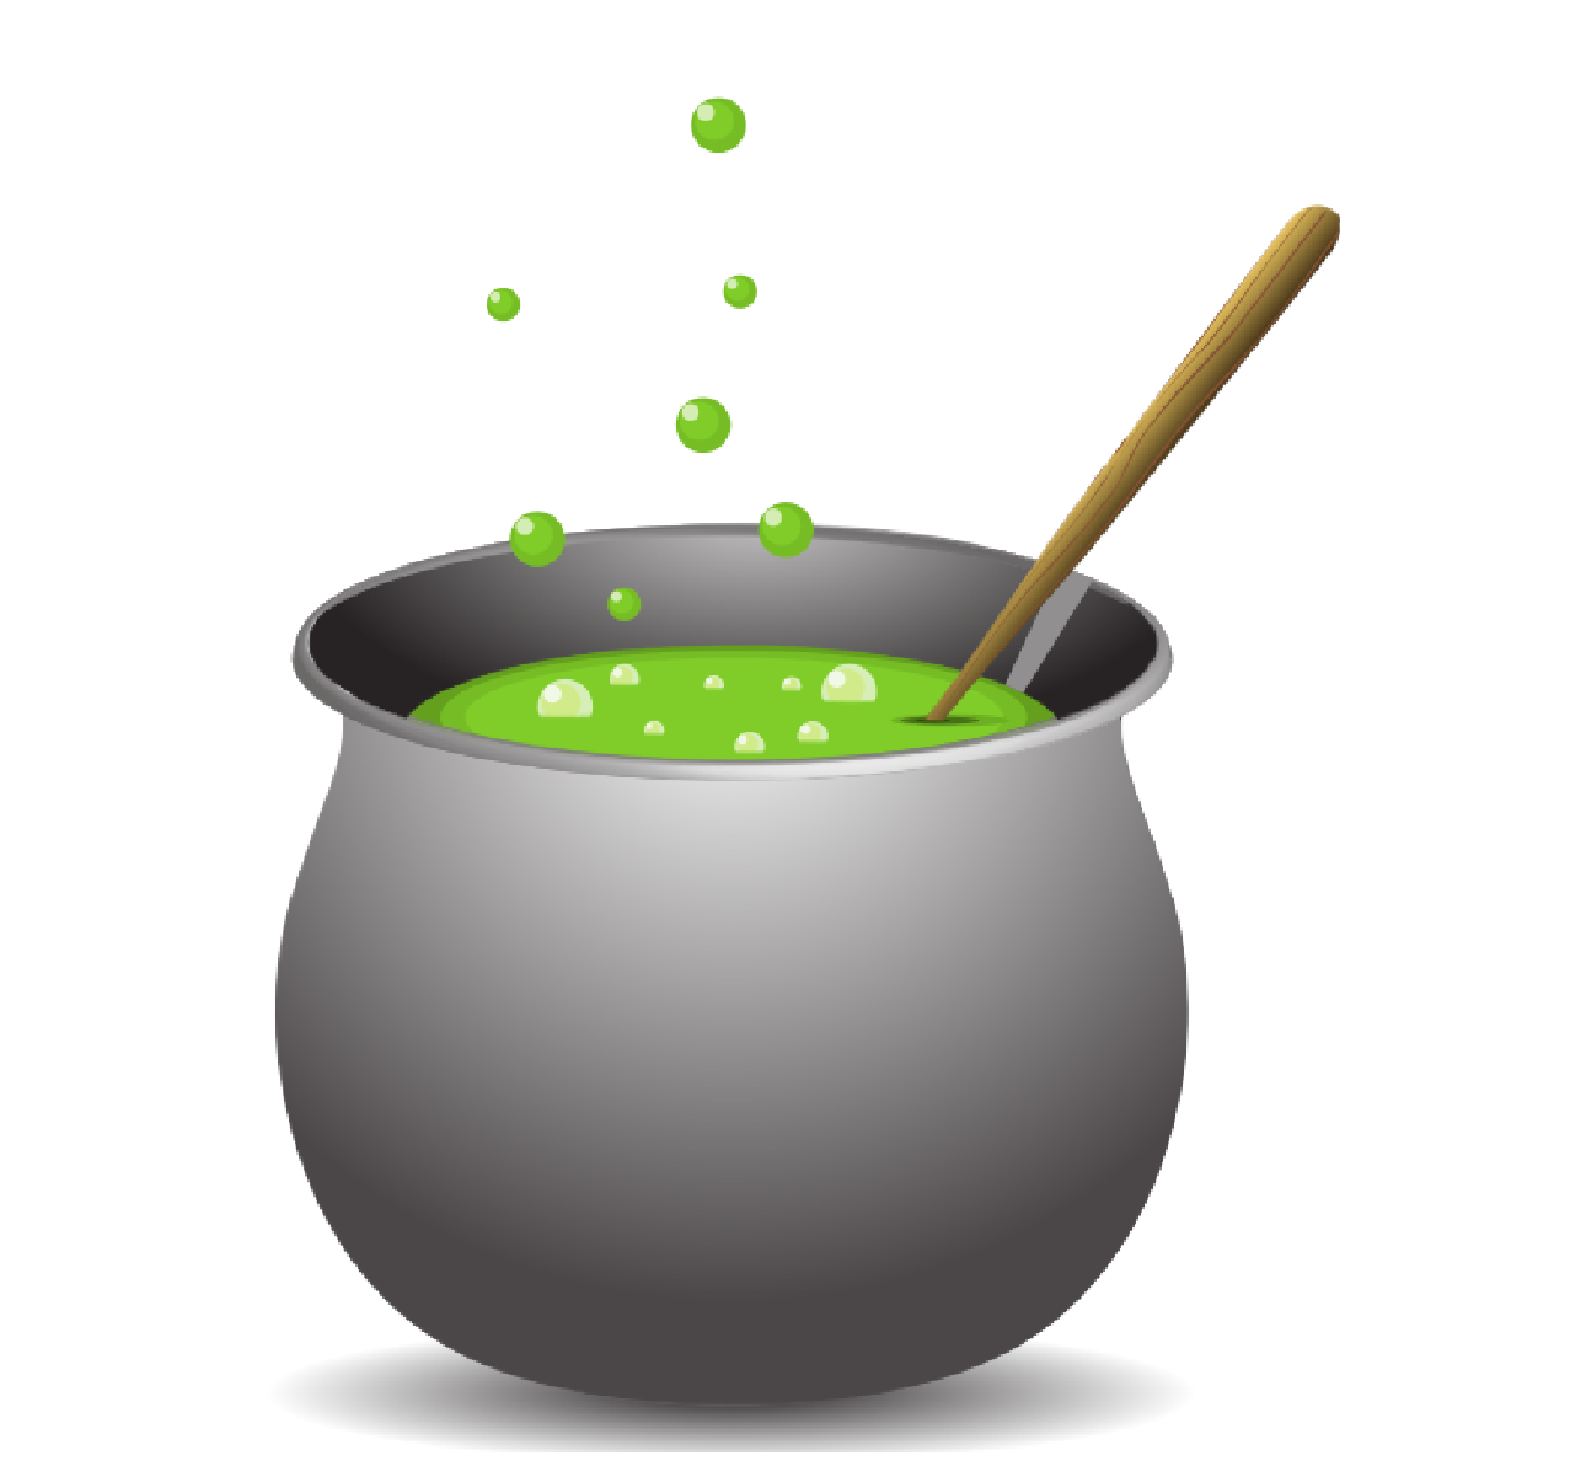
\includegraphics[width = \columnwidth]{img/kociol.eps}
  }
  
\vfill\null
\end{wideslide}

